
\usepackage[all]{nowidow}
\usepackage{siunitx}
\usepackage{multirow}
\usepackage{amsmath}
\usepackage{booktabs}
\usepackage{tabularx}
\usepackage{array}
\usepackage{makecell} % optional (not required below)
\newcolumntype{Y}{>{\raggedright\arraybackslash}X}
\usepackage[most]{tcolorbox}
\usepackage{subcaption}
% \usepackage[hidelinks]{hyperref}
\RequirePackage{doi}
\usepackage{comment}
\usepackage{amssymb}
\usepackage{fancyhdr}
\usepackage{pifont} %dingautolist 
\usepackage{float}
% break urls
% \usepackage{breakurl}
\def\UrlBreaks{\do\/\do-\do_}

\renewcommand{\sectionautorefname}{Section}
\renewcommand{\subsectionautorefname}{Section}
\renewcommand{\subsubsectionautorefname}{Section}
\renewcommand{\appendixautorefname}{Appendix}
% For appendix references
\newcommand{\refappendix}[1]{\hyperref[#1]{Appendix~\ref*{#1}}}
\newcommand{\refethics}[1]{\hyperref[#1]{Ethical Considerations}}
\newcommand{\refopenscience}[1]{\hyperref[#1]{Open Science}}

% \renewcommand{\algorithmautorefname}{Algorithm}

% Prior work comparison table
\usepackage{graphicx}
\newcommand*\rot{\rotatebox{90}}
%Circles
\usepackage{tikz}
\newcommand{\emptypie}{%

\begin{tikzpicture}
 \draw (0,0) circle (.75ex);
\end{tikzpicture}%
}
\newcommand{\pie}[1]{%
\begin{tikzpicture}
 \draw (0,0) circle (.75ex);\fill[rotate=90] (.75ex,0) arc (0:#1:.75ex) -- (0,0) -- cycle;
\end{tikzpicture}%
}
\newcommand{\xmark}{\ding{55}}%

% \usepackage{xspace}
% % Add a period to the end of an abbreviation unless there's one
% % already, then \xspace.
% \makeatletter
% \DeclareRobustCommand\onedot{\futurelet\@let@token\@onedot}
% \def\@onedot{\ifx\@let@token.\else.\null\fi\xspace}

% \def\eg{e.g\onedot}\def\Eg{E.g\onedot}
% \def\ie{i.e\onedot} \def\Ie{I.e\onedot}
% \def\cf{c.f\onedot} \def\Cf{C.f\onedot}
% \def\etc{etc\onedot} \def\vs{vs\onedot}
% \def\wrt{w.r.t\onedot} \def\dof{d.o.f\onedot}
% \def\etal{et al\onedot}
% \makeatother

\newcommand{\todo}[1]{\textcolor{red}{[#1]}}
\newcommand{\subscript}[2]{$#1 _ #2$}

\setlength{\doublerulesep}{2.5pt}

\newif{\ifanonymous}
\anonymoustrue{} % hide or show authors and other parts of the paper that should not appear at submission time


%% Gaps and Open Problem Boxed Frame
\newcommand{\gap}{\textbf{Gap}:}
\newcommand{\openproblem}{\textbf{Open Problem}:}

\usepackage[strict]{changepage}
\usepackage{framed}
\usepackage{color}

\definecolor{cosmiclatte}{rgb}{1.0, 0.97, 0.91}
\definecolor{darkred}{HTML}{AE4132}
\definecolor{lightred}{HTML}{FAD9D5}

% keywords search criteria
\newenvironment{exclusionkeywordbox}{%
  \def\FrameCommand{%
    {\color[HTML]{f8cecc}\vrule width 2pt}%
    \colorbox[HTML]{f8cecc}%
  }%
  \MakeFramed{\advance\hsize-\width\FrameRestore}%
  \noindent\hspace{-4.55pt}%
  \begin{adjustwidth}{}{7pt}%
}
{%
\end{adjustwidth}\endMakeFramed%
}

\newenvironment{keywordbox}{%
  \def\FrameCommand{%
    {\color[HTML]{d5e8d4}\vrule width 2pt}%
    \colorbox[HTML]{d5e8d4}%
  }%
  \MakeFramed{\advance\hsize-\width\FrameRestore}%
  \noindent\hspace{-4.55pt}%
  \begin{adjustwidth}{}{7pt}%
}
{%
\end{adjustwidth}\endMakeFramed%
}

% open problems
\newenvironment{opbox}{%
  \vspace{-8pt}%
  \def\FrameCommand{%
    {\color{darkred}\vrule width 2pt}%
    \colorbox{lightred}%
  }%
  \MakeFramed{\advance\hsize-\width\FrameRestore}%
  \noindent\hspace{-4.55pt}%
  \begin{adjustwidth}{}{2pt}%
  \openproblem%
}
{%
\end{adjustwidth}\endMakeFramed%
\vspace{-8pt}%
}


% gaps
\newenvironment{gapbox}{%
  \def\FrameCommand{%
    {\color{darkgray}\vrule width 2pt}%
    \colorbox{lightgray}%
  }%
  \MakeFramed{\advance\hsize-\width\FrameRestore}%
  \noindent\hspace{-4.55pt}%
  \begin{adjustwidth}{}{7pt}%
  \gap%
}
{%
\end{adjustwidth}\endMakeFramed%
}



% Defense deployment

\newcommand{\dNative}{\ding{108}} % in-browser
\newcommand{\dExt}{\ding{117}} % extension
\newcommand{\dTool}{\ding{109}} % offline/list tool
\newcommand{\dServer}{\ding{115}} % server/network/protocol/OS
\newcommand{\dNo}{\textemdash} % no/unknown industrial defense


% Tracker capabilities

% Circle fills (light pastels)
\definecolor{capIncBg}{HTML}{DBEAFE}
\definecolor{capExeBg}{HTML}{FEE2E2}
\definecolor{capObsBg}{HTML}{FEF3C7}
\definecolor{capStoBg}{HTML}{CCFBF1}
\definecolor{capShaBg}{HTML}{EDE9FE}

% Circle borders
\definecolor{capIncBd}{HTML}{93C5FD}
\definecolor{capExeBd}{HTML}{FCA5A5}
\definecolor{capObsBd}{HTML}{FCD34D}
\definecolor{capStoBd}{HTML}{5EEAD4}
\definecolor{capShaBd}{HTML}{C4B5FD}

\newcommand{\capsym}[3]{%
  \tikz[baseline=-0.55ex]{%
    \node[circle, fill=#1, draw=#2, line width=0.4pt,
          inner sep=0pt, minimum size=2.1ex,
          font=\fontsize{8}{8}\selectfont\bfseries\sffamily,
          text=black]{#3};}}

\newcommand{\symInclusion}{\capsym{capIncBg}{capIncBd}{I}}
\newcommand{\symExecution}{\capsym{capExeBg}{capExeBd}{E}}
\newcommand{\symObservation}{\capsym{capObsBg}{capObsBd}{O}}
\newcommand{\symStorage}{\capsym{capStoBg}{capStoBd}{T}}
\newcommand{\symSharing}{\capsym{capShaBg}{capShaBd}{S}}





% Icons for tracking mechanisms

\newlength{\iconsize}
\setlength{\iconsize}{0.9em}
 
\newcommand{\iconURL}{\raisebox{-0.15em}{
\includegraphics[height=\iconsize]{figures/icons/url.png}}}
\newcommand{\iconFingerprint}{\raisebox{-0.15em}{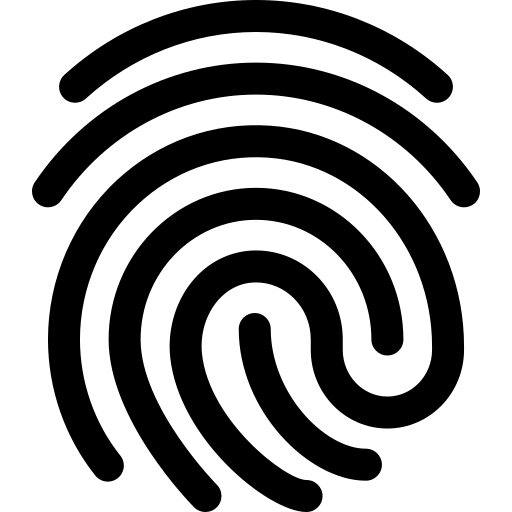
\includegraphics[height=\iconsize]{figures/icons/fingerprint.png}}}
\newcommand{\iconCookie}{\raisebox{-0.15em}{
\includegraphics[height=\iconsize]{figures/icons/cookie.png}}}
\newcommand{\iconJS}{\raisebox{-0.15em}{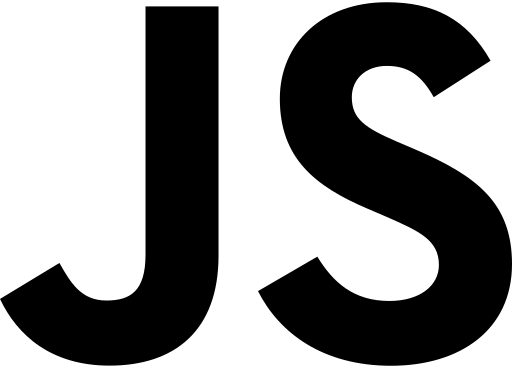
\includegraphics[height=\iconsize]{figures/icons/js.png}}}
\newcommand{\iconPrivacy}{\raisebox{-0.15em}{
\includegraphics[height=\iconsize]{figures/icons/privacy.jpg}}}
\newcommand{\iconBehavioral}{\raisebox{-0.15em}{
\includegraphics[height=\iconsize]{figures/icons/behavioral.png}}}
\newcommand{\iconSC}{\raisebox{-0.15em}{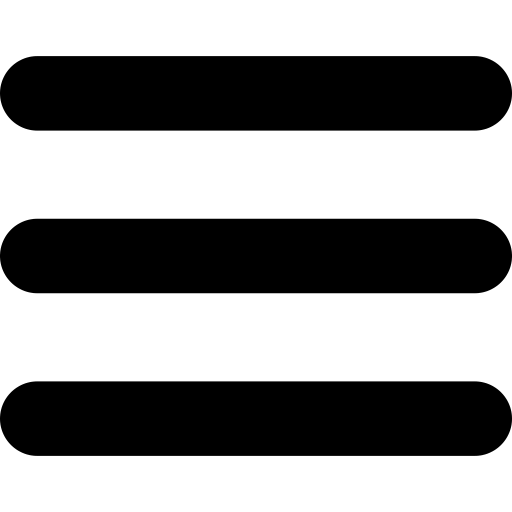
\includegraphics[height=\iconsize]{figures/icons/sc.png}}}

\newcommand{\iconAdBlock}{\raisebox{-0.15em}{\includegraphics[height=\iconsize]{figures/icons/block.png}}}
\newcommand{\iconCNAME}{\raisebox{-0.15em}{\includegraphics[height=\iconsize]{figures/icons/cname.png}}}



\newcommand{\iconBlocklist}{\raisebox{-0.15em}{
\includegraphics[height=\iconsize]{figures/icons/blocklist.png}}}
\newcommand{\iconExtension}{\raisebox{-0.15em}{
\includegraphics[height=\iconsize]{figures/icons/extension.png}}}
\newcommand{\iconTool}{\raisebox{-0.15em}{
\includegraphics[height=\iconsize]{figures/icons/tool.png}}}



% Browser icons
\newcommand{\iconIE}{\raisebox{-0.3em}{
\includegraphics[height=1.6em]{figures/icons/ie.png}}}
\newcommand{\iconEdge}{\raisebox{-0.3em}{
\includegraphics[height=1.6em]{figures/icons/edge.png}}}
\newcommand{\iconFirefox}{\raisebox{-0.3em}{
\includegraphics[height=1.6em]{figures/icons/firefox.png}}}
\newcommand{\iconSafari}{\raisebox{-0.3em}{
\includegraphics[height=1.6em]{figures/icons/safari.png}}}
\newcommand{\iconChrome}{\raisebox{-0.3em}{
\includegraphics[height=1.6em]{figures/icons/chrome.png}}}
\newcommand{\iconBrave}{\raisebox{-0.3em}{
\includegraphics[height=1.6em]{figures/icons/brave.png}}}





% Defense Goals

% Detection and Blocking
\definecolor{cellred}{RGB}{252,235,235}
% Signal Reduction and Obfuscation
\definecolor{cellyellow}{RGB}{255,253,230}
% Regulation compliance
% Incentives
\definecolor{cellpink}{RGB}{243,230,248}
% Expectations
\definecolor{cellblue}{RGB}{230,241,253}
% Responsibilities
\definecolor{cellgreen}{RGB}{232,250,235}



\definecolor{cellempty}{RGB}{242,242,248}
\newcommand{\ec}{\cellcolor{cellempty}}
\newcommand{\rh}{\rule[-0.9em]{0pt}{2.0em}}
\newcommand{\cellsym}[1]{\parbox[c][2.0em][c]{\linewidth}{\centering #1}}




% \usepackage[landscape,margin=0.35in]{geometry}
\usepackage{calc}
\usepackage[table]{xcolor}



% TBD to create a warning at compilation (i.e., to not forget to edit later)
\newcommand{\TBD}[2]{\errmessage{#1}{[#2]}}
% \newcommand{\TBD}[1]{\errmessage{TBD}{\color{red}{[#1]}}}

%% Students
\newcommand{\yash}[1]{\textcolor{red}{[\textbf{Yash Vekaria}: #1]}}
\newcommand{\yohan}[1]{\textcolor{olive}{[\textbf{Yohan Beugin}: #1]}}
\newcommand{\shaoor}[1]{\textcolor{blue}{[\textbf{Shaoor Munir}: #1]}}

%% Professors
\newcommand{\alexandros}[1]{\textcolor{cyan}{[\textbf{AK}: #1]}}
\newcommand{\franzi}[1]{\textcolor{magenta}{[\textbf{Franziska Roesner}: #1]}}
\newcommand{\gunes}[1]{\textcolor{yellow}{[\textbf{Güneş Acar}: #1]}}
\newcommand{\jason}[1]{\textcolor{brown}{[\textbf{Jason Polakis}: #1]}}
\newcommand{\nataliia}[1]{\textcolor{cyan}{[\textbf{Nataliia Bielova}: #1]}}
\newcommand{\nick}[1]{\textcolor{green}{[\textbf{Nick Nikiforakis}: #1]}}
\newcommand{\pierre}[1]{\textcolor{orange}{[\textbf{Pierre Laperdrix}: #1]}}
\newcommand{\sebastian}[1]{\textcolor{pink}{[\textbf{Sebastian Zimmeck}: #1]}}
\newcommand{\steven}[1]{\textcolor{purple}{[\textbf{Steven Englehardt}: #1]}}
\newcommand{\umar}[1]{\textcolor{teal}{[\textbf{Umar Iqbal}: #1]}}
\newcommand{\zubair}[1]{\textcolor{violet}{[\textbf{Zubair Shafiq}: #1]}}


\newcommand{\para}[1]{\smallskip \noindent \textbf{#1}}
\newcommand{\parait}[1]{\smallskip \noindent \textit{#1}}

%Logos affiliations
\newcommand{\ucDavis}{\raisebox{2pt}{
\includegraphics[width=30pt]{figures/logos/uc-davis.pdf}}}
\newcommand{\uwMadison}{
\includegraphics[height=10pt]{figures/logos/uw-madison.pdf}}
\newcommand{\radboud}{
\includegraphics[height=10pt]{figures/logos/radboud.pdf}}
\newcommand{\inria}{
\includegraphics[height=10pt]{figures/logos/inria.pdf}}
\newcommand{\cnrs}{
\includegraphics[height=10pt]{figures/logos/cnrs.pdf}}
\newcommand{\washU}{
\includegraphics[height=10pt]{figures/logos/washU.jpg}}
\newcommand{\ncstate}{\raisebox{2pt}{
\includegraphics[width=30pt]{figures/logos/ncstate.pdf}}}
\newcommand{\stonybrook}{
\includegraphics[height=10pt]{figures/logos/stonybrook.pdf}}
\newcommand{\uic}{
\includegraphics[height=10pt]{figures/logos/uic.pdf}}
\newcommand{\uwashington}{
\includegraphics[height=8pt]{figures/logos/uwashington.pdf}}
\newcommand{\wu}{
\includegraphics[height=10pt]{figures/logos/wu.pdf}}
\newcommand{\independent}{\raisebox{2pt}{$\dagger$}}